
%----------------------------------------------------------------------------------------
% SECTION 1
%----------------------------------------------------------------------------------------

\section{Training Data}
\label{train_data}


%-----------------------------------
% SUBSECTION 1
%-----------------------------------
\subsection{Data simulation}

The spectra were simulated with the Software Sessa v2.2.0 developed by Smekal et al. It uses binding energies from the NIST database and inelastic mean free paths (IMFPs) from various publications and simulations to calculate the spectra. Since version 2.2.0, it also accounts for energy dependence of the IMFP \cite{noauthor_nist_2010}.

As the probing depth of XPS is around 10 nanometers and the information diminishes rapidly after the first few nanometers, the thicknesses used for simulation of the top layer are n $\in$ [1, 2, 3, 4, 5] nm. A second simulation approach was to simulate slow transitions of elements such as seen in migration, oxidation or alloying processes. As shown in \ref{fig:layers} b), two components are used in a mixture across the lateral cross-section. While one component decreases from 100\%, the other one increases symmetrically.

\begin{figure}
    \centering
    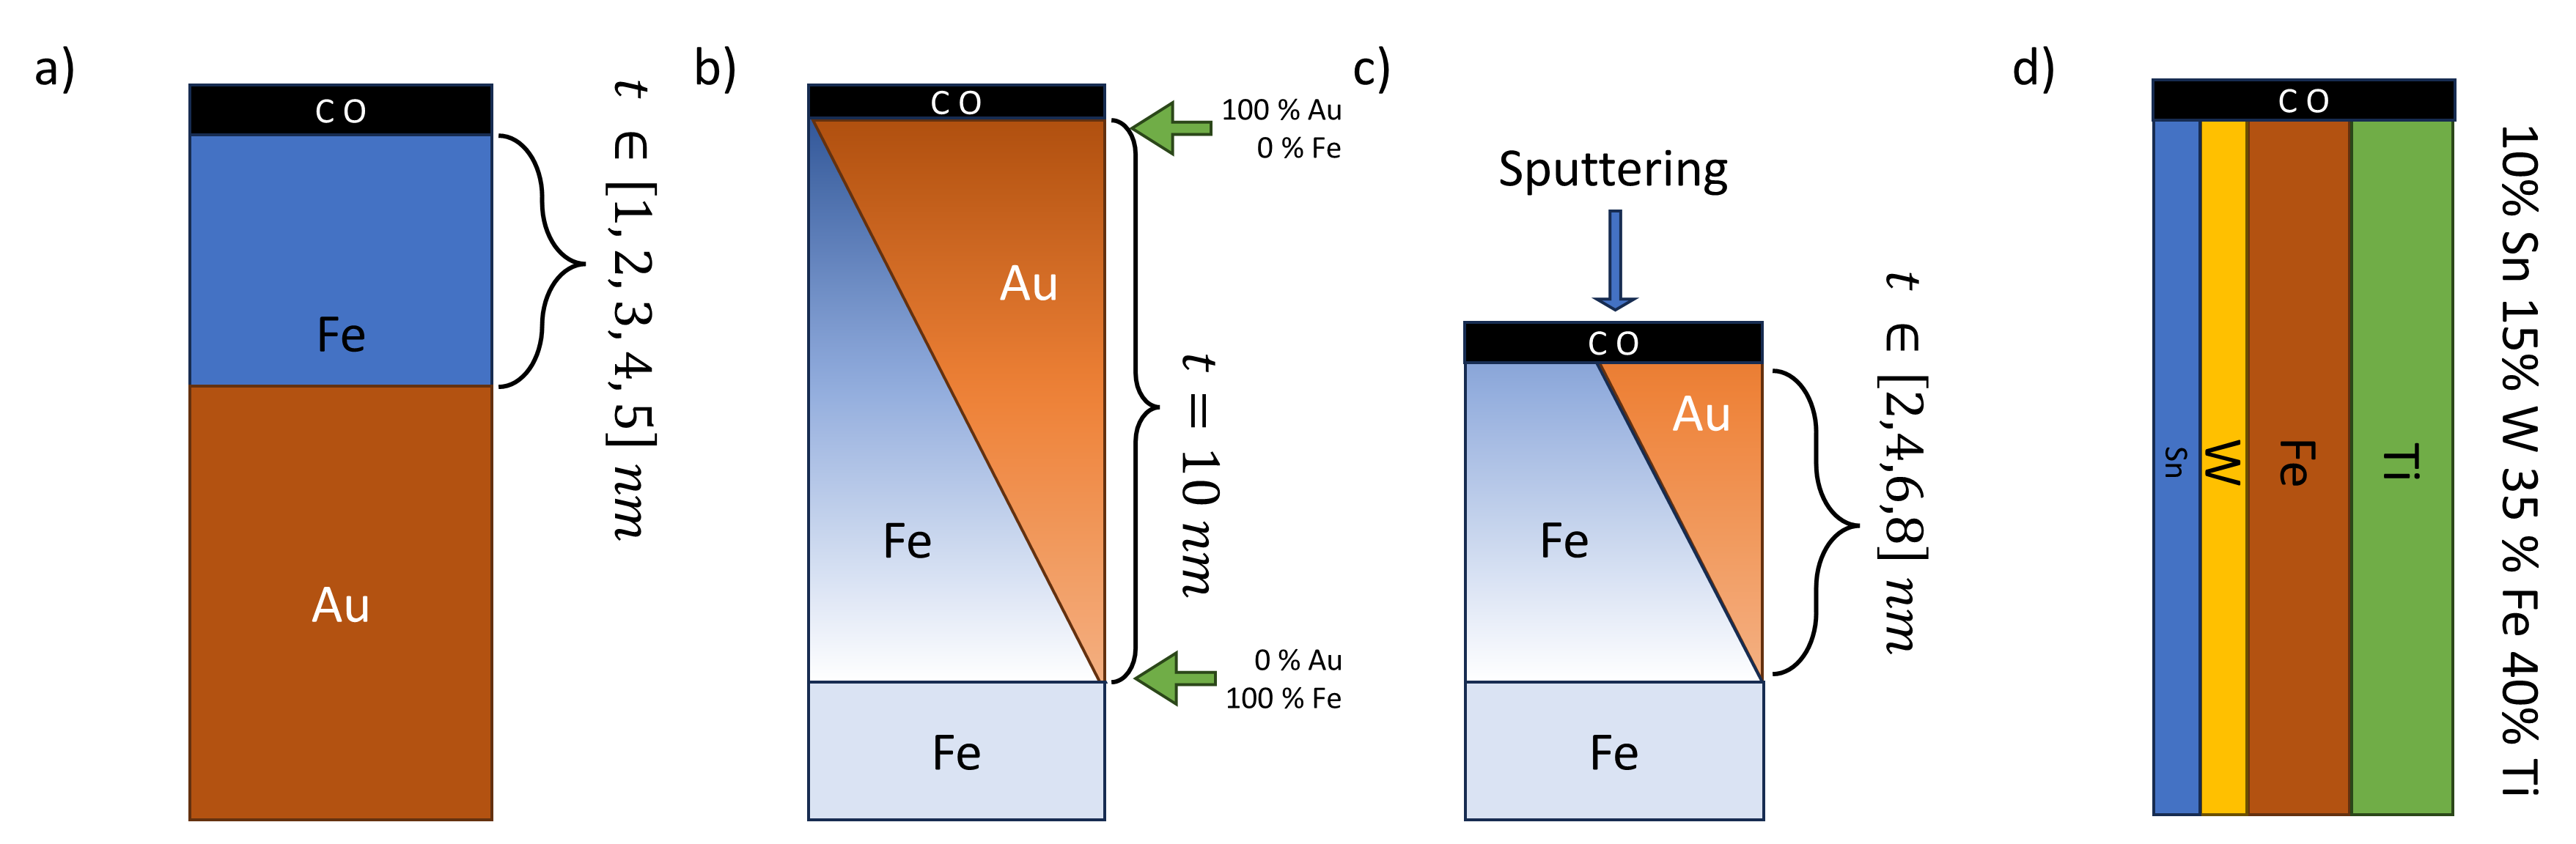
\includegraphics[width=\textwidth]{Figures/layers.png}
    \caption{Simulation of different layered systems a) Separated layers with defined top layer thickness, b) Top layer with a concentration gradient and thickness 10nm, c) Sputtered version of b) where the top layer thickness is reduced, d) Multi-component one-layer system}
    \label{fig:layers}
\end{figure}


The spectra simulated are using two components from all elements (n=81), thus 6561 permutations. With the five thicknesses, we obtain 32805 spectra for each experimental setup a) and b)+c).
The contamination layer is often seen on uncleaned samples but, as discussed, does not resemble a factual layer in XPS analysis. As the contamination has diverse provenance, datasets were constructed with and without a contamination layer. They are denoted as cont. and clean, respectively. Finally, both datasets were used to provide the model with variations of contaminated and clean samples, which is denoted as mixcont. 
To achieve a similar carbon and oxide content as experimental data (because of environmental influences), there is a carbon and oxide layer with thickness of triangular distribution (12-24, mode 15) Angstrom on top. 

To simulate, the CLI feature of Sessa was used. It allows users to interact with the software through a file of commands which are then subsequently read. The commands were first saved to a text-file and then processed with Sessa using the python subprocess module. To allow diverse simulation properties, classes for Experiments and Layers were defined. Furthermore, functions for the simulation, finding and setting chemical shifts, as well as writing the session file were programmed. The corresponding code can be found in \ref{ApendixA}.

Because the Sessa software didn't allow reading the chemical shift database from the command line interface, the NIST database was webscraped and saved as a readable database \ref{}.  

Python-Wrapper, Databases of Sessa, etc., X-Y-axis, carbon / oxygen layer, etc.

%-----------------------------------
% SUBSECTION 2
%-----------------------------------

\subsection{Data preprocessing}

Each spectra was max-normalized using equation \ref{eqn:normalize}, where each component $x$ is divided by the maximum of the spectra. Using the max-normalization ensures that any background-shift of the whole spectrum is kept as a feature.

\begin{equation}
    x' = \frac{x}{max(x)}
\label{eqn:normalize}
\end{equation}

Additionally to the normalization, 0.3 \% relative noise was added to mimick the noise usually observed in XPS spectral data.

